% !TeX root = ../main.tex
% Add the above to each chapter to make compiling the PDF easier in some editors.
\section{\texorpdfstring{\ac{ITM} on a one-dimensional acoustic planar wave}{ITM on a one-dimensional acoustic planar wave}}\label{section:ITMAcoustic}
In this section, we calculate the analytical solution for a one-dimensional acoustic wave when an \ac{ITM} is applied from $t_{ITM}^-$ to $t_{ITM}^+$.
For this, we consider a one-dimensional acoustic equation ~\parencite[Sec. 2.8]{leveque_2002} linearized about the motionless state
\begin{align}
    \begin{split}
        p_t + K_0u_x = 0, \\
        u_t + \frac{1}{\rho_0}p_x = 0 .\\
    \end{split}
\end{align}
where $p$ is the pressure perturbation, $K_0$ is the bulk modulus of the material and $u$ is the velocity perturbation. 
This can be written in consolidated matrix vector form as done for first order hyperbolic systems of equations as follows
\begin{align}
    \begin{split}
        \frac{\partial }{\partial t}
    \begin{bmatrix}
        p \\
        u
    \end{bmatrix} + 
    \begin{bmatrix}
        0 & K_0 \\
        \frac{1}{\rho_0} & 0 \\
    \end{bmatrix}
    \frac{\partial }{\partial x}
    \begin{bmatrix}
        p \\
        u
    \end{bmatrix} = 0 .
    \end{split}
    \label{eq:acoustic}
\end{align}

The flux matrix of equation \ref{eq:acoustic} has two eigenvalues
\begin{align}
    \begin{split}
        \lambda_1 = -c_0, \quad \lambda_2 = c_0,
    \end{split}
\end{align}
where 
\begin{align}
    \begin{split}
        c_0 = \sqrt{\frac{K_0}{\rho_0}}
    \end{split}
\end{align}
is the speed of sound. Waves can propagate in either direction with this speed. The eigenvectors for this coefficient matrix are
\begin{align}
    \begin{split}
        r^1 = \begin{bmatrix}
            -\rho_0 c_0 \\
            1
        \end{bmatrix}, \quad
        r^2 = \begin{bmatrix}
            \rho_0 c_0 \\
            1
        \end{bmatrix}.
    \end{split}
\end{align}

The impedance as mentioned in section \ref{section:ITMTheory} is defined as
\begin{equation}
    Z_0 = \rho_0 c_0.
\end{equation}
\par Using these parameters, ~\parencite[Sec. 2.8]{leveque_2002} calculates the solution of the acoustic equation depending on the initial conditions $p^0(x), u^0(x)$ as:
\begin{align}
    \begin{split}
        p(x,t) &= \frac{1}{2}\left[p^0\left(x + c_0t\right) + p^0\left(x - c_0t\right)\right] - \frac{Z_0}{2}\left[u^0\left(x+c_0t\right) - u^0\left(x-c_0t\right)\right], \\
        u(x,t) &= -\frac{1}{2Z_0}\left[p^0\left(x+c_0t\right) - p^0\left(x-c_0t\right)\right] + \frac{1}{2}\left[u^0\left(x+c_0t\right) + u^0\left(x-c_0t\right)\right] .
    \end{split}
    \label{eq:solutionacoustic}
\end{align}

We use this solution to find the analytical solution of a 1D acoustic wave after the \ac{ITM} is applied in two different ways. First we ensure we use initial conditions which give rise to only one forward wave. We simply use a sinusoidal wave multiplied with one eigenvector $r^2$.
This defines our initial conditions as
\begin{align}
    \begin{split}
        p^0\left(x\right) &= \rho_0c_0 \cos\left(kx\right), \\
        u^0\left(x\right) &= \cos\left(kx\right)
    \end{split}
    \label{eq:initialconditions}
\end{align}

where $k$ is the wave number of the wave. To ensure that our domain is periodic, we defined our domain to be between two wavelengths, i.e., from 
$\left[-\frac{\pi}{k}, \frac{\pi}{k}\right]$. The energy of the system is defined in this domain as ~\parencite{Kopriva2021}

\begin{equation}
     E_1 = \int_{-\frac{\pi}{k}}^{\frac{\pi}{k}} \left(\frac{1}{2K}p^2 + \frac{1}{2}\rho u^2\right) dx,
    \label{eq:energy}
\end{equation}
which simplifies to
\begin{equation}
    E_1 = \frac{\pi\rho_0}{k},
\end{equation}
for phase 1. Energy defined in equation \ref{eq:energy} is conserved for a particular phase as the system of equations are conservative for every phase ~\parencite{Kopriva2021}. 

\subsection{\texorpdfstring{Impedance Changing \ac{ITM}}{Impedance Changing ITM}}\label{section:impedancechangingITM}
Using the conditions given by equation \ref{eq:initialconditions}, we calculate the solution at $t_{ITM}^-$ and use them as initial conditions for the new equation where the material properties are changed.
In this case, we modify the material properties such that the velocities are scaled while the impedance also changes. This is achieved by modifying the bulk modulus while keeping the density constant. Using \ref{eq:solutionacoustic}, we get the initial conditions for the next phase of the simulation$\left(t_{ITM}^- \leq t \leq t_{ITM}^+ \right)$ at $t_{ITM}^-$ as
\begin{align}
    \begin{split}
        p^0_{t_{ITM}^-}\left(x\right) &= c_0 \rho_0 \cos\left(kx - c_0kt_{ITM}^-\right), \\
        u^0_{t_{ITM}^-}\left(x\right) &= \cos\left(kx - c_0kt_{ITM}^-\right) .
    \end{split}
\end{align}

We now use these initial conditions and equation \ref{eq:solutionacoustic} with the updated wave velocity and constant density to get the evolved solution for $t_{ITM}^- \leq t \leq t_{ITM}^+ $. We used~\parencite{sagemath} to perform the arithmetic simplifications. We obtain the solution for this period as
\begin{align}
    \begin{split}
        p_{2}\left(x, t\right) &= -\frac{1}{2} \left(n-1\right)c_0\rho_0 \cos\left(kx + c_0knt - \left(c_0kn + c_0k\right)t_{ITM}^-\right) \\
        &+ \frac{1}{2} \left(n+1\right)c_0\rho_0\cos\left(kx - c_0knt + \left(c_0kn - c_0k\right)t_{ITM}^-\right), \\
        u_{2}\left(x, t\right) &= \frac{1}{2}\left(n-1\right)\cos\left(kx + c_0knt - \left(c_0kn + c_0k\right)t_{ITM}^-\right)\\
        &+ \frac{1}{2}\left(n+1\right)\cos\left(kx - c_0knt + \left(c_0kn-c_0k\right)t_{ITM^-}\right)
    \end{split}
\end{align}
where n is the velocity scaling factor. We now use these expressions to calculate the energy as we have already done in equation \ref{eq:energy}. This gives us the energy in the second phase, i.e., $t_{ITM}^- \leq t \leq t_{ITM}^+ $ to be
\begin{equation}
    E_2 = \frac{1}{2}\frac{\left(1 + n^2\right)\pi \rho_0}{kn^2} .
\end{equation}

This shows that the energy drops when the velocity is scaled up. We then check the relative drop in energy for different scaling factors and see that it asymptotes to 0.5 for higher scaling factors. The variation of the ratio with the scaling factor can be seen in figure \ref{fig:ratio1}.

\begin{figure}[!htpb]
    \centering
    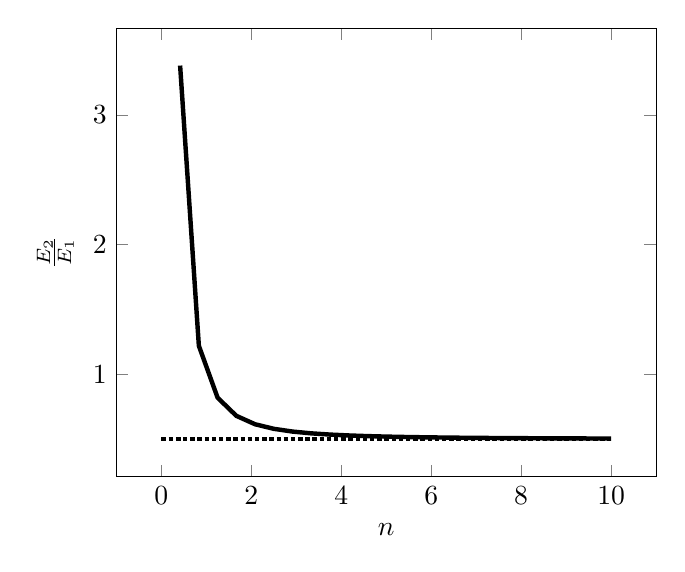
\begin{tikzpicture}[scale=1.0]
        \begin{axis}[
            ylabel = $\frac{E_2}{E_1}$,
            xlabel = $n$]
            \addplot[domain=0:10, black, ultra thick]{0.5*(1+x*x)/(x*x)};
            \addplot[domain=0:10, black, ultra thick, densely dotted]{0.5};
        \end{axis}
    \end{tikzpicture}
    \caption{Relative Energy $\left(\frac{E_2}{E_1}\right)$ in $t_{ITM}^- \leq t \leq t_{ITM}^+$. }
    \label{fig:ratio1}
\end{figure}

Now, the velocity is scaled back to its initial value at $t=t_{ITM}^+$. By defining $\tau = t_{ITM}^+ - t_{ITM}^-$, a similar calculation is performed to acquire the
solution for the final phase, i.e., $t \geq t_{ITM}^+$, and the resulting solution is
\begingroup
\allowdisplaybreaks
\begin{align}
    \begin{split}
        p_3\left(x, t\right) & = -\frac{{\frac{1}{4}c_{0}\rho_{0}\left( -n^{2} + 1\right)} \cos\left(k x + c_{0} k t - 2 \, c_{0} k \mathit{t_{ITM}^-} - {\left(c_{0} k n + c_{0} k\right)} \tau\right)}{n} \\
        & - \frac{{\frac{1}{4}c_0\rho_0\left(n^{2} - 1\right)} \cos\left(k x + c_{0} k t - 2 \, c_{0} k \mathit{t_{ITM}^-} + {\left(c_{0} k n - c_{0} k\right)} \tau\right)}{n} \\
        & - \frac{{\frac{1}{4}c_0\rho_0\left(n^{2} - 2n + 1\right)} \cos\left(kx -c_{0} k t + {\left(c_{0} k n + c_{0} k\right)} \tau\right)}{n} \\
        & - \frac{{\frac{1}{4}c_0\rho_0\left(-n^{2} - 2n - 1\right)} \cos\left(kx-c_{0} k t - {\left(c_{0} k n - c_{0} k\right)} \tau\right)}{n}, \\
        u_3\left(x, t\right) & =  -\frac{{\frac{1}{4}\left(n^{2} - 1\right)} \cos\left( k x + c_{0} k t - 2 \, c_{0} k \mathit{t_{ITM}^-} - {\left(c_{0} k n + c_{0} k\right)} \tau\right)}{n} \\
        & - \frac{{\frac{1}{4}\left(-n^{2} + 1\right)} \cos\left(kx + c_{0} k t - 2 \, c_{0} k \mathit{t_{ITM}^-} + {\left(c_{0} k n - c_{0} k\right)} \tau\right)}{n} \\
        & - \frac{{\frac{1}{4}\left(n^{2} - 2n + 1\right)} \cos\left(kx -c_{0} k t + {\left(c_{0} k n + c_{0} k\right)} \tau\right)}{n} \\
        & - \frac{{\frac{1}{4}\left(-n^{2} - 2n - 1\right)} \cos\left(kx -c_{0} k t - {\left(c_{0} k n - c_{0} k\right)} \tau\right)}{n} .
    \end{split}
\end{align}
\endgroup

Using these quantities, we now calculate the energy using the equation \ref{eq:energy}
\begin{equation}
    E_3 = -\pi \rho_0\frac{{\left(1 + n^{4} - 2 \, n^{2}\right)} \cos^{2}\left(c_{0} k n \tau\right) - {\left(1 + n^{4}\right)}}{2 \, k n^{2}}.
\end{equation}

The final energy $E_3$ is dependent on the parameters: $k, n, \tau$ and is bounded as

\begin{equation}
    \frac{\pi \rho_0}{K} \leq E_3 \leq \frac{\pi \rho_0}{2K}\left[n^2 + \frac{1}{n^2}\right] .
\end{equation}

This demonstrates that the application of \ac{ITM} leads to a change in the energy of our system. We compare the worst case scenario, i.e., what would be the maximum energy increase after the ITM is applied. For that,
 we take the upper bound and plot the ratio $\frac{E_3}{E_1}$ with $n$ as we did before in figure \ref{fig:ratio2}.

\begin{figure}[!htpb]
    \centering
    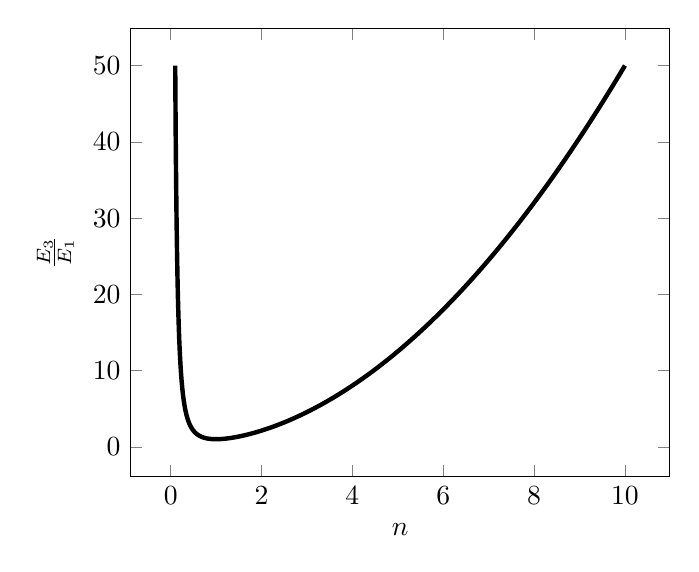
\begin{tikzpicture}[scale=1.0]
        \begin{axis}[
            ylabel = $\frac{E_3}{E_1}$,
            xlabel = $n$]
            \addplot[domain=0.1:10, samples=1001, black, ultra thick]{0.5*((1/x)^2 + x^2)};
        \end{axis}
    \end{tikzpicture}
    \caption{Maximum Relative Energy$\left(\frac{E_3}{E_1}\right)$ in $t \geq t_{ITM}^+$}
    \label{fig:ratio2}
\end{figure}

The minimum value for this energy jump lies at $n=1$, which means no velocity scaling and no reflections. This particular scenario does not offer any practical utility
or relevance to our objective.

\subsection{\texorpdfstring{Constant Impedance \ac{ITM}}{Constant Impedance ITM}}
We know that there is no reflected wave in space interfaces when the impedance stays constant~\parencite[Sec 9.7]{leveque_2002}. Here, we test out the same with a time interface, i.e., we perform \ac{ITM} such that the velocities scale but the impedance stays constant. This is achieved by scaling the wave speed by $n$ and the density by $\frac{1}{n}$.
Similar to section \ref{section:impedancechangingITM}, we choose the initial conditions as
\begin{align}
    \begin{split}
        p^0\left(x\right) &= Z_0 \cos\left(kx\right), \\
        u^0\left(x\right) &= \cos\left(kx\right) .
    \end{split}
    \label{eq:initialconditions2}
\end{align}

Using these parameters, the energy is once again computed as in equation \ref{eq:energy} and is found to be
\begin{equation}
    E_1 = \frac{\pi Z_0}{c_0 k} .
\end{equation}

Using the conditions given in equation \ref{eq:initialconditions2}, we calculate the solution at $t_{ITM}^-$ and use them as initial conditions for the new equation where the wave velocities are scaled.
In this case, we scale the velocities such that the impedance does not change. This is achieved by scaling the density down. Using \ref{eq:solutionacoustic}, we get the initial conditions for the next phase of the simulation$\left(t_{ITM}^- \leq t \leq t_{ITM}^+ \right)$ at $t_{ITM}^-$ as
\begin{align}
    \begin{split}
        p^0_{t_{ITM}^-}\left(x\right) &= Z_0 \cos\left(kx - c_0kt_{ITM}^-\right), \\
        u^0_{t_{ITM}^-}\left(x\right) &= \cos\left(kx - c_0kt_{ITM}^-\right) .
    \end{split}
\end{align}

We now use these as the initial conditions and equation \ref{eq:solutionacoustic} with the updated wave velocity and constant density to get the evolved solution for $t_{ITM}^- \leq t \leq t_{ITM}^+ $. 
We used ~\parencite{sagemath} to perform the simplifications for the arithmetic. We obtain the solution for this period as
\begin{align}
    \begin{split}
        p_{2}\left(x, t\right) &= Z_{0} \cos\left(kx -c_{0} k n t + {\left(c_{0} k n - c_{0} k\right)} \mathit{t_{ITM}^-}\right), \\
        u_{2}\left(x, t\right) &= \cos\left(kx -c_{0} k n t + {\left(c_{0} k n - c_{0} k\right)} \mathit{t_{ITM}^-} \right) .
    \end{split}
\end{align}
where n is the velocity scaling factor. We now use these expressions to calculate the energy using equation \ref{eq:energy}. This gives us the energy in the second phase, i.e., $t_{ITM}^- \leq t \leq t_{ITM}^+ $ to be
\begin{equation}
    E_2 = \frac{\pi z_{0}}{c_{0} k n} .
\end{equation}

We obverse that there is no extra reflected wave and the wave speed is just increased with a phase shift and that the energy is directly scaled down by the velocity scaling factor.

% \begin{figure}
%     \centering
%     \begin{tikzpicture}[scale=1.0]
%         \begin{axis}[
%             ylabel = $\frac{E_2}{E_1}$,
%             xlabel = $n$]
%             \addplot[domain=0:10, black, ultra thick]{0.5*(1+x*x)/(x*x)};
%         \end{axis}
%     \end{tikzpicture}
%     \caption{Relative Energy in $t_{ITM}^- \leq t \leq t_{ITM}^+$}
%     \label{fig:ratio1}
% \end{figure}

Now, the velocity is scaled down again to its original value at $t=t_{ITM}^+$ and defining $\tau = t_{ITM}^+ - t_{ITM}^-$, we do a similar calculation to obtain the solution for the final phase, i.e., $t \geq t_{ITM}^+$ as
\begin{align}
    \begin{split}
        p_3\left(x, t\right) & = Z_{0} \cos\left(kx - c_{0} k t - {\left(c_{0} k n - c_{0} k\right)} \tau\right) , \\
        u_3\left(x, t\right) & =  \cos\left(kx - c_{0} k t - {\left(c_{0} k n - c_{0} k\right)} \tau\right) . 
    \end{split}
\end{align}

Using these quantities, we now calculate the energy using equation \ref{eq:energy}
\begin{equation}
    E_3 = \frac{\pi Z_0}{c_0 k} ,
\end{equation}
which is equal to $E_1$. This shows that there is no final energy increase when the impedance is kept constant. The final solution also has no reflected wave and has the same wave speed as the initial wave and has a phase shift in time. This confirms that even in time interfaces, similar to space interfaces there is no reflection.

% \begin{align}
%     \begin{split}
%         \left(\left(\begin{array}{rrrr}
%             1 & 1 & 0 & 0 \\
%             -\frac{k_{1}}{\rho_{0} \sqrt{\frac{K_{0} k_{1}^{2} + K_{0} k_{2}^{2} + K_{0} k_{3}^{2}}{\rho_{0}}}} & \frac{k_{1}}{\rho_{0} \sqrt{\frac{K_{0} k_{1}^{2} + K_{0} k_{2}^{2} + K_{0} k_{3}^{2}}{\rho_{0}}}} & 1 & 0 \\
%             -\frac{k_{2}}{\rho_{0} \sqrt{\frac{K_{0} k_{1}^{2} + K_{0} k_{2}^{2} + K_{0} k_{3}^{2}}{\rho_{0}}}} & \frac{k_{2}}{\rho_{0} \sqrt{\frac{K_{0} k_{1}^{2} + K_{0} k_{2}^{2} + K_{0} k_{3}^{2}}{\rho_{0}}}} & 0 & 1 \\
%             -\frac{k_{3}}{\rho_{0} \sqrt{\frac{K_{0} k_{1}^{2} + K_{0} k_{2}^{2} + K_{0} k_{3}^{2}}{\rho_{0}}}} & \frac{k_{3}}{\rho_{0} \sqrt{\frac{K_{0} k_{1}^{2} + K_{0} k_{2}^{2} + K_{0} k_{3}^{2}}{\rho_{0}}}} & -\frac{k_{1}}{k_{3}} & -\frac{k_{2}}{k_{3}}
%             \end{array}\right)\right)
%     \end{split}
% \end{align}

\section{\texorpdfstring{\ac{ITM}}{ITM} on a 3D acoustic planar wave}\label{section:3DITMAcoustic}
In this section, we calculate the analytical solution for a 3D Acoustic wave when an \ac{ITM} is applied from $t_{ITM}^-$ to $t_{ITM}^+$.

To do this, we consider a three dimensional acoustic equation linearised over the stationary state, where $p$ is the pressure perturbation, $K_0$ is the bulk
modulus of the material and $u,\,v,\,w$ are the velocity perturbations in $x,\,y,\,z$ respectively. This can be written in consolidated matrix vector form as done for first order hyperbolic systems of equations as

\begin{align}
    \begin{split}
        \frac{\partial}{\partial t}\mathbf{q} + \mathbf{A}\frac{\partial}{\partial x}\mathbf{q} + \mathbf{B}\frac{\partial}{\partial y}\mathbf{q} + 
        \mathbf{C}\frac{\partial}{\partial z}\mathbf{q} = 0,
    \end{split}
    \label{eq:3Dacoustic}
\end{align}
where
\begin{align}
    \begin{split}
        \mathbf{q} = \begin{bmatrix}
            p \\
            u \\
            v \\
            w 
        \end{bmatrix}, \quad
        \mathbf{A} = \begin{bmatrix}
            0 & K_0 & 0 & 0 \\
            \frac{1}{\rho_0} & 0 & 0 & 0 \\
            0 & 0 & 0 & 0 \\
            0 & 0 & 0 & 0 \\
        \end{bmatrix}, \quad
        \mathbf{B} = \begin{bmatrix}
            0 & 0 & K_0 & 0 \\
            0 & 0 & 0 & 0 \\
            \frac{1}{\rho_0} & 0 & 0 & 0 \\
            0 & 0 & 0 & 0 \\
        \end{bmatrix}, \quad
        \mathbf{C} = \begin{bmatrix}
            0 & 0 & 0 & K_0 \\
            0 & 0 & 0 & 0 \\
            0 & 0 & 0 & 0 \\
            \frac{1}{\rho_0} & 0 & 0 & 0 \\
        \end{bmatrix} \quad .
    \end{split}
\end{align}

We assume an ansatz of 
\begin{equation}
    \mathbf{q}\left(\mathbf{x}, t\right) = \mathbf{q_0} \cos\left(\mathbf{k}\cdot\mathbf{x} - \omega t\right),
\end{equation}
where $\mathbf{k}=\left(k_1, k_2, k_3\right)$ is the wave number of the planar wave. Using the derivatives of equation \ref{eq:3Dacoustic},
\begin{align}
    \begin{split}
    \frac{\partial \mathbf{q}}{\partial t} &= \omega \mathbf{q_0} \sin\left(\mathbf{k}\cdot\mathbf{x} - \omega t\right), \\
    \frac{\partial \mathbf{q}}{\partial x} &= -k_1 \mathbf{q_0} \sin\left(\mathbf{k}\cdot\mathbf{x} - \omega t\right), \\
    \frac{\partial \mathbf{q}}{\partial y} &= -k_2 \mathbf{q_0} \sin\left(\mathbf{k}\cdot\mathbf{x} - \omega t\right), \\
    \frac{\partial \mathbf{q}}{\partial z} &= -k_3 \mathbf{q_0} \sin\left(\mathbf{k}\cdot\mathbf{x} - \omega t\right).
\end{split}
\end{align}

Substituting these back in the equation we get
\begin{align}
    \begin{split}
        \left(\omega - \mathbf{A}k_1 - \mathbf{B}k_2 - \mathbf{C}k_3\right)\mathbf{q_0}\sin\left(\mathbf{k}\cdot\mathbf{x} - \omega t\right) = 0.
    \end{split}
\end{align}

Dividing by $\sin\left(\mathbf{k}\cdot\mathbf{x} - \omega t\right)$ and rearranging the terms, we get
\begin{align}
    \begin{split}
        \left(\mathbf{A}k_1 + \mathbf{B}k_2 + \mathbf{C}k_3\right)\mathbf{q_0} = \omega \mathbf{q_0}
    \end{split}
\end{align}

This shows that $\omega$ is an eigenvalue of $\mathbf{\hat{A}} = \mathbf{A}k_1 + \mathbf{B}k_2 + \mathbf{C}k_3$ and $\mathbf{q_0}$ is an eigenvector. The modified matrix $\mathbf{\hat{A}}$ would then be
\begin{align}
    \begin{split}
    \mathbf{\hat{A}} = \left(\begin{array}{rrrr}
0 & K_{0} k_{1} & K_{0} k_{2} & K_{0} k_{3} \\
\frac{k_{1}}{\rho_{0}} & 0 & 0 & 0 \\
\frac{k_{2}}{\rho_{0}} & 0 & 0 & 0 \\
\frac{k_{3}}{\rho_{0}} & 0 & 0 & 0
\end{array}\right)
    \end{split}
\end{align}
with the set of eigenvalues after replacing $\sqrt{\frac{K_{0}}{\rho_{0}}}$ with $c$
\begin{align}
    \begin{split}
        \omega_1 = -c \sqrt{k_{1}^{2} + k_{2}^{2} + k_{3}^{2}}, \quad
        \omega_2 = 0, \quad
        \omega_3 = 0, \quad 
        \omega_4 = c \sqrt{k_{1}^{2} + k_{2}^{2} + k_{3}^{2}},
    \end{split}
\end{align}
and the eigenvectors after replacing $\rho_0 \sqrt{\frac{K_0}{\rho_0}}$ with $Z_0$,
\begin{align}
    \begin{split}
    \mathbf{r_1} = \begin{bmatrix}
        1 \\
-\frac{k_{1}}{Z_0 \sqrt{k_{1}^{2} + k_{2}^{2} + k_{3}^{2}}} \\
-\frac{k_{2}}{Z_0 \sqrt{k_{1}^{2} + k_{2}^{2} + k_{3}^{2}}} \\
-\frac{k_{3}}{Z_0 \sqrt{k_{1}^{2} + k_{2}^{2} + k_{3}^{2}}}
        \end{bmatrix}, \quad
        \mathbf{r_2} = \begin{bmatrix}
            0 \\
1 \\
0 \\
-\frac{k_{1}}{k_{3}}
            \end{bmatrix}, \quad
            \mathbf{r_3} = \begin{bmatrix}
                0 \\
                0 \\
                1 \\
                -\frac{k_{2}}{k_{3}}
                \end{bmatrix}, \quad
                \mathbf{r_4} = \begin{bmatrix}
                    1 \\
\frac{k_{1}}{Z_0 \sqrt{k_{1}^{2} + k_{2}^{2} + k_{3}^{2}}} \\
\frac{k_{2}}{Z_0 \sqrt{k_{1}^{2} + k_{2}^{2} + k_{3}^{2}}} \\
\frac{k_{3}}{Z_0 \sqrt{k_{1}^{2} + k_{2}^{2} + k_{3}^{2}}}
                    \end{bmatrix} .
    \end{split}
\end{align}

For the sake of simplicity, we choose $\left(k_1,k_2,k_3\right) = \left(k,0,0\right)$ inducing our wave to travelling along the x-axis. This makes our eigenvalues
\begin{align}
    \begin{split}
        \omega_1 = -k c, \quad
        \omega_2 = 0, \quad
        \omega_3 = 0, \quad
        \omega_4 = k c .
    \end{split}
\end{align}

We get our eigenvectors as
\begin{align}
    \begin{split}
    \mathbf{r_1} = \begin{bmatrix}
        1 \\
-\frac{1}{Z_0} \\
0 \\
0
        \end{bmatrix}, \quad
        \mathbf{r_2} = \begin{bmatrix}
            0 \\
0 \\
0 \\
1
            \end{bmatrix}, \quad
            \mathbf{r_3} = \begin{bmatrix}
                0 \\
                0 \\
                1 \\
                0
                \end{bmatrix}, \quad
                \mathbf{r_4} = \begin{bmatrix}
                    1 \\
                    \frac{1}{Z_0} \\
                    0 \\
                    0                    
                \end{bmatrix} .
    \end{split}
\end{align}

We pick an initial condition that enforces that the wave travels in only one direction at $t=0$ i.e.,
\begin{align}
    \begin{split}
        \mathbf{q_1}\left(\mathbf{x}, t\right) = \begin{bmatrix}
            1 \\
            \frac{1}{Z_0} \\
            0 \\
            0
            \end{bmatrix} \cos\left(kx - k ct\right) .
    \end{split}
\end{align}

This wave form satifies our \ac{PDE} in equation \ref{eq:3Dacoustic}.

Now, applying ITM in phase 2 leads to a modified $\mathbf{\hat{A}}$, as we make specific changes to our material properties, specifically replacing $K_0$ with $n^2K_0$. The modified matrix would then be

\begin{align}
    \begin{split}
    \mathbf{\hat{A}_2} = \begin{bmatrix}
        0 & K_{0} n^{2} & 0 & 0 \\
\frac{1}{\rho_{0}} & 0 & 0 & 0 \\
0 & 0 & 0 & 0 \\
0 & 0 & 0 & 0
    \end{bmatrix},
    \end{split}
\end{align}
with eigenvalues
\begin{align}
    \begin{split}
    \omega_1^2 = -n k c, \quad
    \omega_2^2 = 0, \quad
    \omega_3^2 = 0, \quad
    \omega_4^2 = n k c,
\end{split}
\end{align}
and eigenvectors
\begin{align}
    \begin{split}
    \mathbf{r_1^2} = \begin{bmatrix}
        1 \\
-\frac{1}{n Z_0} \\
0 \\
0
        \end{bmatrix}, \quad
        \mathbf{r_2^2} = \begin{bmatrix}
            0 \\
0 \\
0 \\
1
            \end{bmatrix}, \quad
            \mathbf{r_3^2} = \begin{bmatrix}
                0 \\
                0 \\
                1 \\
                0
                \end{bmatrix}, \quad
                \mathbf{r_4^2} = \begin{bmatrix}
                    1 \\
                    \frac{1}{n Z_0} \\
                    0 \\
                    0                    
                \end{bmatrix}.
    \end{split}
\end{align}

At $t = t_{ITM}^-$, the solution is 
\begin{align}
    \begin{split}
        \mathbf{q}\left(\mathbf{x}, t_{ITM}^-\right) = \begin{bmatrix}
            1 \\
            \frac{1}{Z_0} \\
            0 \\
            0
            \end{bmatrix} \cos\left(kx - k c t_{ITM}^-\right) .
    \end{split}
    \label{eq:initphase2}
\end{align}

We use this solution as the initial condition for the next phase with the modified \ac{PDE}. We split this into a linear sum of the eigenvectors of the new flux matrix
as 
\begin{equation}
    \mathbf{q_1}\left(\mathbf{x}, t_{ITM}^-\right) = \alpha_1^2 \mathbf{r_1^2} + \alpha_2^2 \mathbf{r_2^2} + \alpha_3^2 \mathbf{r_3^2} + \alpha_4^2 \mathbf{r_4^2},
    \label{eq:linearsum}
\end{equation}
with
\begin{align}
    \begin{split}
        \alpha_1^2 &= \frac{1}{2}\cos\left(kx - k c t_{ITM}^-\right) \left(1 - n\right), \\
        \alpha_2^2 &= 0, \\
        \alpha_3^2 &= 0, \\
        \alpha_4^2 &= \frac{1}{2}\cos\left(kx - k c t_{ITM}^-\right) \left(1 + n\right) .
    \end{split}
\end{align}

\parencite[Sec 18.5]{leveque_2002} states that the solution for a linear hyperbolic system with an eigenvector $\mathbf{\hat{q}}$ and an initial condition $\mathbf{q_0} = \mathbf{\hat{q}} \, f\left(\mathbf{n} \cdot \mathbf{x}\right)$
and eigenvalues of the system would be $q\left(\mathbf{x}, t\right) = \mathbf{\hat{q}} \, f\left( \mathbf{n} \cdot \mathbf{x} - s t\right)$. 
Using initial conditions from equation \ref{eq:initphase2} and the linear combindation of the eigenvectors, we get the solution for the second phase as

\begin{align}
    \begin{split}
        \mathbf{q_2}\left(\mathbf{x}, t\right) &= 
        \frac{1}{2} \begin{bmatrix}
            1 \\
            -\frac{1}{nZ_0} \\
            0 \\
            0
        \end{bmatrix} \left(1 - n\right) \cos\left(kx +nk c \left(t - t_{ITM}^-\right) - k c t_{ITM}^-\right) \\ 
        &+ \frac{1}{2} 
        \begin{bmatrix}
            1 \\
            \frac{1}{nZ_0} \\
            0 \\
            0
        \end{bmatrix} \left(1 + n\right) \cos\left(kx - nk c \left(t - t_{ITM}^-\right) - k c t_{ITM}^-\right) .
    \end{split}
\end{align}

We define the duration of \ac{ITM} as $\tau = t_{ITM}^+ - t_{ITM}^-$, this makes the initial conditions for our final phase as
\begin{align}
    \begin{split}
        \mathbf{q_2}\left(\mathbf{x}, t_{ITM}^+\right) &= 
        \frac{1}{2} \begin{bmatrix}
            1 \\
            -\frac{1}{nZ_0} \\
            0 \\
            0
        \end{bmatrix} \left(1 - n\right) \cos\left(kx +nk c \tau - k c t_{ITM}^-\right) \\ 
        &+ \frac{1}{2} 
        \begin{bmatrix}
            1 \\
            \frac{1}{nZ_0} \\
            0 \\
            0
        \end{bmatrix} \left(1 + n\right) \cos\left(kx - nk c \tau - k c t_{ITM}^-\right) .
    \end{split}
    \label{eq:initphase3}
\end{align}

The flux matrix, eigenvalues and eigenvectors of the final phase are identical to those of the first phase. We use the initial conditions in equation \ref{eq:initphase3}
and split the initial conditions into a linear sum of the eigenvectors of the flux matrix similar to what we have done in equation \ref{eq:linearsum}. 
We get the new coefficients for this phase as
\begin{align}
    \begin{split}
        \frac{2n}{n^2 - 1} \alpha_1^3\left(kx\right) &=  {\cos\left(k x\right) \sin\left(k n \tau c\right) \sin\left(k \mathit{t_{ITM}^-} c\right) - \cos\left(k \mathit{t_{ITM}^-} c\right) \sin\left(k n \tau c\right) \sin\left(k x\right)}, \\
        \alpha_2^3 &= 0, \\
        \alpha_3^3 &= 0, \\
        {2n} \alpha_4^3 \left(kx\right) &= {\left(2 \, n \cos\left(k n \tau c\right) \cos\left(k \mathit{t_{ITM}^-} c\right) - {\left(n^{2} + 1\right)} \sin\left(k n \tau c\right) \sin\left(k \mathit{t_{ITM}^-} c\right)\right)} \cos\left(k x\right) \\
        &+ {\left({\left(n^{2} + 1\right)} \cos\left(k \mathit{t_{ITM}^-} c\right) \sin\left(k n \tau c\right) + 2 \, n \cos\left(k n \tau c\right) \sin\left(k \mathit{t_{ITM}^-} c\right)\right)} \sin\left(k x\right) .
    \end{split}
\end{align}

The final solution for the third phase is then given by
\begin{align}
    \begin{split}
        \mathbf{q_2}\left(\mathbf{x}, t\right) = \begin{bmatrix}
            1 \\
            -\frac{1}{Z_0} \\
            0 \\
            0
        \end{bmatrix} \alpha_1^3 \left(kx + kc \left(t - t_{ITM}^+\right)\right) + 
        \begin{bmatrix}
            1 \\
            \frac{1}{Z_0} \\
            0 \\
            0
        \end{bmatrix} \alpha_4^3 \left(kx - kc \left(t - t_{ITM}^+\right)\right) .
    \end{split}
\end{align}

This shows that the final wave solution obtained after \ac{ITM} has both a forward and a backward going component. This is similar to the solution obtained in section \ref{section:impedancechangingITM}.